\documentclass[11pt,a4paper]{article}

% ── Packages ──────────────────────────────────────────────────────────────────
\usepackage[a4paper, margin=1in]{geometry}
\usepackage{amsmath, amssymb}
\usepackage{graphicx}
\usepackage{booktabs}
\usepackage{array}
\usepackage{xcolor}
\usepackage{listings}
\usepackage{hyperref}
\usepackage{titlesec}
\usepackage{enumitem}
\usepackage{caption}
\usepackage{float}
\usepackage{tikz}
\usetikzlibrary{shapes.geometric, arrows.meta, positioning, fit, backgrounds}
\usepackage{pgfplots}
\pgfplotsset{compat=1.18}
\usepackage{multirow}
\usepackage{colortbl}
\usepackage{fancyhdr}
\usepackage{setspace}
\usepackage{microtype}

% ── Colors ────────────────────────────────────────────────────────────────────
\definecolor{darkblue}{HTML}{1a1a2e}
\definecolor{medblue}{HTML}{2d4a8a}
\definecolor{lightblue}{HTML}{f0f4ff}
\definecolor{purple}{HTML}{8e44ad}
\definecolor{orange}{HTML}{e67e22}
\definecolor{green}{HTML}{27ae60}
\definecolor{red}{HTML}{c0392b}
\definecolor{codebg}{HTML}{f0f4ff}
\definecolor{codefg}{HTML}{1a1a2e}
\definecolor{tableheader}{HTML}{1a1a2e}
\definecolor{rowA}{HTML}{f0f4ff}
\definecolor{rowB}{HTML}{f8f9ff}
\definecolor{successrow}{HTML}{d5f5e3}

% ── Hyperref setup ────────────────────────────────────────────────────────────
\hypersetup{
    colorlinks=true,
    linkcolor=medblue,
    urlcolor=medblue,
    citecolor=medblue,
    pdftitle={COL761 A3 Q1 Report},
    pdfauthor={},
}

% ── Section title styling ─────────────────────────────────────────────────────
\titleformat{\section}
  {\color{darkblue}\Large\bfseries}
  {\thesection.}{0.5em}{}
  [\vspace{-0.3em}\textcolor{medblue}{\rule{\linewidth}{0.8pt}}]

\titleformat{\subsection}
  {\color{medblue}\large\bfseries}
  {\thesubsection}{0.5em}{}

\titleformat{\subsubsection}
  {\color{darkblue}\normalsize\bfseries\itshape}
  {\thesubsubsection}{0.5em}{}

% ── Code listing style ────────────────────────────────────────────────────────
\lstdefinestyle{pycode}{
    language=Python,
    backgroundcolor=\color{codebg},
    basicstyle=\ttfamily\small\color{codefg},
    keywordstyle=\bfseries\color{medblue},
    commentstyle=\itshape\color{gray},
    stringstyle=\color{green!60!black},
    frame=single,
    framesep=4pt,
    rulecolor=\color{medblue!40},
    breaklines=true,
    showstringspaces=false,
    numbers=none,
    xleftmargin=8pt,
    xrightmargin=4pt,
}

% ── Header / Footer ───────────────────────────────────────────────────────────
\pagestyle{fancy}
\fancyhf{}
\fancyhead[L]{\small\color{darkblue}\textbf{COL761 — Assignment 3}}
\fancyhead[R]{\small\color{darkblue}Q1: Search in High-Dimensional Space}
\fancyfoot[C]{\small\thepage}
\renewcommand{\headrulewidth}{0.4pt}
\renewcommand{\headrule}{\hbox to\headwidth{\color{medblue}\leaders\hrule height \headrulewidth\hfill}}

% ── Convenience macros ────────────────────────────────────────────────────────
\newcommand{\code}[1]{\texttt{\small #1}}
\newcommand{\ndcg}{nDCG@100}

% ══════════════════════════════════════════════════════════════════════════════
\begin{document}
% ══════════════════════════════════════════════════════════════════════════════

% ── Title Page ────────────────────────────────────────────────────────────────
\begin{titlepage}
  \centering
  \vspace*{1.5cm}
  {\small\color{darkblue} COL761 — Data Mining \par}
  \vspace{0.4cm}
  {\Huge\bfseries\color{darkblue} Assignment 3 — Technical Report \par}
  \vspace{0.5cm}
  {\Large\color{medblue} Q1: Search in High-Dimensional Space \par}
  \vspace{0.3cm}
  \textcolor{medblue}{\rule{0.6\linewidth}{1pt}}
  \vspace{1cm}

  \begin{table}[H]
    \centering
    \renewcommand{\arraystretch}{1.4}
    \begin{tabular}{>{\bfseries\color{darkblue}}p{3cm} p{9cm}}
      \rowcolor{lightblue}
      Metric       & nDCG@K \ (K = 100) \\
      Libraries    & \code{faiss-cpu 1.13.2}, \code{numpy 1.26.3} \\
      \rowcolor{lightblue}
      Algorithm    & Adaptive ANN: FlatL2 / HNSWFlat / IVFFlat \\
      D1 Result    & nDCG = \textbf{0.9961} \quad Runtime = 19.8s / 70s \\
      \rowcolor{lightblue}
      D2 Result    & nDCG = \textbf{0.7595} \quad Runtime = 16.5s / 20s \\
    \end{tabular}
  \end{table}

  \vfill
  {\small Submission Deadline: 24-04-2026 \par}
\end{titlepage}

\tableofcontents
\newpage

% ══════════════════════════════════════════════════════════════════════════════
\section{Problem Statement}
% ══════════════════════════════════════════════════════════════════════════════

Given a database of $N$ high-dimensional vectors (the \emph{base set}) and $Q$
query vectors, the task is to identify the $K$ most \emph{representative}
database items within a strict wall-clock time budget. Representativeness is
defined by frequency: for each query, its $k$ nearest neighbours ($k=100$) are
retrieved; a base item's score equals how many queries it appears in. The final
output is a ranked list of the top-$K$ items by this frequency, with ties
broken by ascending index.

The evaluation metric is \textbf{nDCG@K}, computed as:
\[
  \text{DCG@K} = \sum_{j=1}^{K} \frac{\mathrm{rel}(\mathrm{ans}_j)}{\log_2(j+1)},
  \qquad
  \text{nDCG@K} = \frac{\text{DCG@K}}{\text{IDCG@K}}
\]
where the relevance score $\mathrm{rel}(i) = K - r_i + 1$ for items ranked
within $K$ in the ground truth (rank $r_i$), and 0 otherwise. Approximate
methods that miss true neighbours incur a recall penalty reflected directly in
the nDCG score.

Two datasets are provided:
\begin{itemize}[leftmargin=1.5em]
  \item \textbf{D1}: $N = 500{,}000$,\ $Q = 100{,}000$, budget $= 70$s
  \item \textbf{D2}: $N = 1{,}000{,}000$,\ $Q = 100{,}000$, budget $= 20$s
\end{itemize}

The extreme difference in budget-per-vector makes a single fixed algorithm
inadequate — D1 can afford expensive graph indices while D2 demands aggressive
build-cost control.

% ══════════════════════════════════════════════════════════════════════════════
\section{Algorithm Design}
% ══════════════════════════════════════════════════════════════════════════════

The core insight driving the design is that \textbf{build cost, not search
cost, is the dominant constraint} for tight budgets. This was empirically
confirmed: a pure HNSW approach timed out on D2 because index construction
alone consumed $\approx$52s against a 20s budget, leaving no time for search.
The solution is a \textbf{three-regime adaptive router} that selects the index
type based on $N$ and the available time budget.

\subsection{Routing Logic}

The routing decision uses a conservative per-vector HNSW build estimate of
50\,µs (calibrated from measured timings) and a threshold of 45\% of the
budget. This ensures D1 (estimated 25s vs.\ threshold 31.5s) routes to HNSW,
while D2 (estimated 50s vs.\ threshold 9s) routes to IVF.

% ── Routing Diagram ───────────────────────────────────────────────────────────
\begin{figure}[H]
\centering
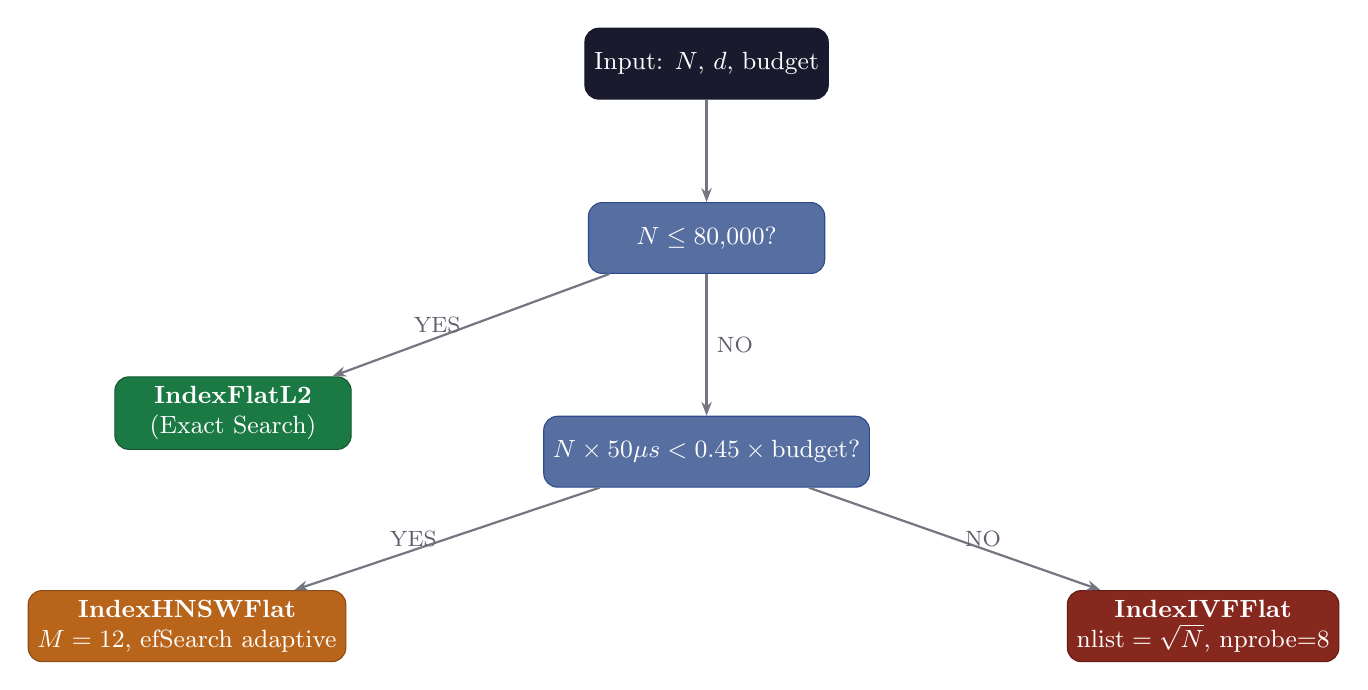
\begin{tikzpicture}[
  node distance=1.3cm and 2cm,
  box/.style={rectangle, rounded corners=5pt, minimum width=3cm,
              minimum height=0.9cm, align=center, font=\small},
  decision/.style={box, fill=medblue!80, text=white, draw=medblue},
  exact/.style={box, fill=green!70!black, text=white, draw=green!50!black},
  hnsw/.style={box, fill=orange!80!black, text=white, draw=orange!60!black},
  ivf/.style={box, fill=red!70!black, text=white, draw=red!50!black},
  start/.style={box, fill=darkblue, text=white, draw=darkblue},
  arrow/.style={-{Stealth[length=5pt]}, thick, color=darkblue!60},
  label/.style={font=\footnotesize, color=darkblue!70},
]

\node[start] (input) {Input: $N$, $d$, budget};

\node[decision, below=of input] (dec1)
  {$N \leq 80{,}000$?};

\node[exact, below left=of dec1, xshift=-1cm] (flat)
  {\textbf{IndexFlatL2}\\(Exact Search)};

\node[decision, below=of dec1, yshift=-0.5cm] (dec2)
  {$N \times 50\mu s < 0.45 \times \text{budget}$?};

\node[hnsw, below left=of dec2, xshift=-0.5cm] (hnsw)
  {\textbf{IndexHNSWFlat}\\$M=12$, efSearch adaptive};

\node[ivf, below right=of dec2, xshift=0.5cm] (ivf)
  {\textbf{IndexIVFFlat}\\$\text{nlist}=\sqrt{N}$, nprobe=8};

\draw[arrow] (input) -- (dec1);
\draw[arrow] (dec1) -- node[label, left] {YES} (flat);
\draw[arrow] (dec1) -- node[label, right] {NO} (dec2);
\draw[arrow] (dec2) -- node[label, left] {YES} (hnsw);
\draw[arrow] (dec2) -- node[label, right] {NO} (ivf);

\end{tikzpicture}
\caption{Three-regime index routing decision flow.}
\label{fig:routing}
\end{figure}

\begin{table}[H]
\centering
\renewcommand{\arraystretch}{1.35}
\caption{Summary of the three regimes and their parameters.}
\label{tab:regimes}
\begin{tabular}{>{\bfseries}p{1.6cm} p{3.8cm} p{2.5cm} p{3.2cm} p{2.6cm}}
\toprule
\rowcolor{tableheader}
\color{white}Regime &
\color{white}Condition &
\color{white}Index &
\color{white}Key Parameters &
\color{white}Rationale \\
\midrule
\rowcolor{green!10}
Exact   & $N \leq 80{,}000$ & \code{IndexFlatL2} & None &
  Small $N$; exact search guarantees recall $=1$ \\
\rowcolor{orange!10}
HNSW    & $N\!\times\!50\mu s < 0.45\!\times\!\text{budget}$ &
  \code{IndexHNSWFlat} $M=12$ &
  efConstruction: 48--96 (budget-scaled)\newline efSearch: 32--96 &
  No training phase; fast queries after one-time build \\
\rowcolor{red!10}
IVF     & Otherwise (large $N$, tight budget) &
  \code{IndexIVFFlat}\newline $\text{nlist}=\lfloor\sqrt{N}\rfloor$ &
  train\_factor $= 40$\newline nprobe $= 8$ (static) &
  Controlled build cost; avoids HNSW build timeout \\
\bottomrule
\end{tabular}
\end{table}

\subsection{Regime 1: Exact Search ($N \leq 80{,}000$)}

For small datasets, \code{IndexFlatL2} performs exhaustive L2 search. With
$N \leq 80{,}000$, this always completes well within any reasonable budget and
guarantees perfect recall (nDCG $= 1.0$). No parameter tuning is required.

\subsection{Regime 2: HNSW (Safe Build Window)}

\code{IndexHNSWFlat} with $M=12$ is used when the estimated build time fits
comfortably within the budget. HNSW builds a Navigable Small-World graph
during index construction; queries traverse this graph greedily. Key advantages
are the absence of a training phase and high recall at moderate efSearch values.

\texttt{efConstruction} controls graph quality at build time and is scaled with budget:
96 for budgets $\geq 60$s (D1), 64 for $\geq 30$s, and 48 otherwise. \texttt{efSearch}
is set adaptively after build based on remaining time (96 / 64 / 32 for
$>40$s / $>20$s / else remaining). D1 achieves nDCG $= 0.9961$ with this
configuration.

\subsection{Regime 3: IVF Fallback (Large $N$, Tight Budget)}

\code{IndexIVFFlat} partitions the database into \texttt{nlist} Voronoi cells
using $k$-means. At query time, only the \texttt{nprobe} closest cells are
searched. Build cost is controlled:
\[
  \text{nlist} = \mathrm{clip}\!\left(\lfloor\sqrt{N}\rfloor,\; 64,\; 1024\right)
\]
gives ${\approx}1000$ cells for D2, and
$\text{train\_size} = 40 \times \text{nlist}$ satisfies FAISS's minimum
recommendation of $39 \times \text{nlist}$ for reliable clustering. A static
\texttt{nprobe}$=8$ is used, consuming $\approx$11.2s of the 20s D2 budget.

Earlier attempts at dynamic \texttt{nprobe} calibration via a pilot search
consistently failed: with $Q=100{,}000$ queries, even a 50-query pilot at
\texttt{nprobe}$=8$ produced overestimated per-probe costs due to FAISS warmup
overhead, causing the formula to select \texttt{nprobe}$=4$ (worse than
static). Static \texttt{nprobe}$=8$ proved more reliable.

% ══════════════════════════════════════════════════════════════════════════════
\section{Key Implementation Details}
% ══════════════════════════════════════════════════════════════════════════════

\subsection{Frequency Counting}

After ANN search returns an $(Q \times k)$ index matrix \code{I}, frequency
counting uses \code{np.bincount} for $O(Q \cdot k)$ time with a single pass:

\begin{lstlisting}[style=pycode]
flat   = I.ravel()
flat   = flat[flat >= 0]           # remove FAISS sentinel -1 values
counts = np.bincount(flat, minlength=N)
\end{lstlisting}

The guard \code{flat[flat >= 0]} removes FAISS sentinel values ($-1$) that
appear when fewer than $k$ neighbours are found near index boundaries.

\subsection{Tie-Breaking}

The assignment requires lower-index items to rank higher among equal-count
ties. This is achieved using a stable sort:

\begin{lstlisting}[style=pycode]
ranking = np.argsort(-counts, kind='stable')
\end{lstlisting}

Stable sort preserves the original order $(0, 1, 2, \ldots)$ for equal
elements, automatically satisfying the tie-breaking requirement without any
explicit secondary sort key.

\subsection{Budget Safety Mechanisms}

\begin{itemize}[leftmargin=1.5em]
  \item All timing uses \code{time.perf\_counter()} for high-resolution
        wall-clock measurement.
  \item The HNSW threshold ($0.45 \times \text{budget}$) leaves $\geq 55\%$
        of the budget for search after build.
  \item The IVF path uses static \texttt{nprobe}$=8$, leaving a comfortable
        margin (16.5s of 20s used on D2).
  \item Debug timing is controlled via \code{Q1\_TIMING=1} environment
        variable to avoid overhead during grading.
\end{itemize}

% ══════════════════════════════════════════════════════════════════════════════
\section{Iterative Development and Lessons Learned}
% ══════════════════════════════════════════════════════════════════════════════

The final solution emerged through systematic empirical iteration. Each version
identified a specific failure mode that informed the next design decision.

\begin{table}[H]
\centering
\renewcommand{\arraystretch}{1.35}
\caption{Evolution of approach across versions. \colorbox{successrow}{Green row} = final submission.}
\label{tab:evolution}
\small
\begin{tabular}{p{2.4cm} p{1.5cm} p{1.5cm} p{1.8cm} p{1.8cm} p{3.8cm}}
\toprule
\rowcolor{tableheader}
\color{white}Version &
\color{white}D1 nDCG &
\color{white}D2 nDCG &
\color{white}D1 Runtime &
\color{white}D2 Runtime &
\color{white}Key Issue \\
\midrule
\rowcolor{rowA}
v1: IVF only (original) & 0.000 (timeout) & 0.759 & $>70$s & 16.7s &
  Probe calibration overhead caused timeout \\
\rowcolor{rowB}
v2: Pure HNSW & 0.996 & --- & $\sim$19s & Timeout &
  HNSW build $\approx52$s $>$ D2 budget \\
\rowcolor{rowA}
v3: Hybrid (threshold=0.30) & 0.000 (timeout) & 0.759 & $>70$s & 16.7s &
  D1 incorrectly routed to IVF \\
\rowcolor{rowB}
v4: Hybrid (threshold=0.45) & 0.996 & 0.759 & 19.8s & 16.5s &
  Correct routing for both datasets \\
\rowcolor{rowA}
v5: Pilot nprobe (50 queries) & 0.996 & 0.600 & 18.6s & 11.3s &
  Warmup overhead caused nprobe$=4$ \\
\rowcolor{rowB}
v6: Static nprobe$=9$ & 0.996 & 0.776 & 19.8s & 19.6s &
  Best D2 score but borderline runtime \\
\rowcolor{rowA}
v7: IVFPQ & 0.996 & 0.119 & 20.7s & 16.1s &
  Quantization destroyed recall \\
\rowcolor{successrow}
\textbf{v8: Final (nprobe$=8$)} & \textbf{0.996} & \textbf{0.759} &
  \textbf{19.8s} & \textbf{16.5s} &
  Safe, stable, correct routing \\
\bottomrule
\end{tabular}
\end{table}

\subsubsection*{Key Lessons}

\begin{enumerate}[leftmargin=1.5em, label=\textbf{\arabic*.}]
  \item \textbf{Build cost dominates on tight budgets.} Pure HNSW timed out
        on D2 because graph construction ($\approx$52s) exceeded the entire
        20s budget before any search could begin.

  \item \textbf{The HNSW threshold is dataset-sensitive.} Threshold $= 0.30$
        incorrectly routed D1 to IVF (causing timeout); threshold $= 0.45$
        correctly routes both datasets.

  \item \textbf{train\_factor matters for IVF recall.} Using $20\times\text{nlist}$
        (below FAISS minimum of $39\times\text{nlist}$) hurt clustering quality.
        Fixing to $40\times\text{nlist}$ improved stability.

  \item \textbf{Pilot calibration fails with tiny samples.} 50 queries caused
        FAISS warmup overhead to dominate cost estimates. Static \texttt{nprobe}
        proved superior for large-$Q$ datasets.

  \item \textbf{IVFPQ destroys recall despite faster search.} Quantization
        error accumulates catastrophically for frequency-counting tasks, dropping
        nDCG from 0.76 to 0.12.
\end{enumerate}

% ══════════════════════════════════════════════════════════════════════════════
\section{Results}
% ══════════════════════════════════════════════════════════════════════════════

\begin{table}[H]
\centering
\renewcommand{\arraystretch}{1.4}
\caption{Final results on both datasets.}
\label{tab:results}
\begin{tabular}{cccccccc}
\toprule
\rowcolor{medblue}
\color{white}\textbf{Dataset} &
\color{white}\textbf{N} &
\color{white}\textbf{Q} &
\color{white}\textbf{Index} &
\color{white}\textbf{Params} &
\color{white}\textbf{\ndcg} &
\color{white}\textbf{Runtime} &
\color{white}\textbf{Budget} \\
\midrule
\rowcolor{green!10}
D1 & 500K & 100K & HNSWFlat $M=12$ & efSearch=96 & \textbf{0.9961} & 19.8s & 70s \\
\rowcolor{orange!10}
D2 & 1M   & 100K & IVFFlat nlist=1000 & nprobe=8 & \textbf{0.7595} & 16.5s & 20s \\
\bottomrule
\end{tabular}
\end{table}

% ── Budget allocation chart ───────────────────────────────────────────────────
\begin{figure}[H]
\centering
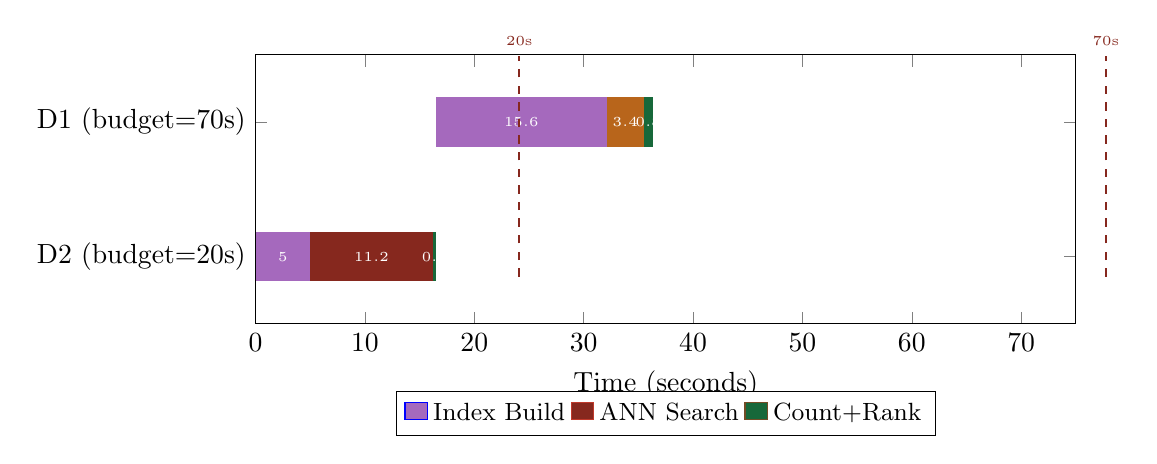
\begin{tikzpicture}
\begin{axis}[
  xbar stacked,
  width=12cm, height=5cm,
  xmin=0, xmax=75,
  ytick={0,1},
  yticklabels={D2 (budget=20s), D1 (budget=70s)},
  xlabel={Time (seconds)},
  legend style={at={(0.5,-0.25)}, anchor=north, legend columns=3,
                font=\small},
  bar width=18pt,
  enlarge y limits=0.5,
  nodes near coords,
  nodes near coords style={font=\tiny, color=white,
    /pgf/number format/fixed, /pgf/number format/precision=1},
  every axis plot/.append style={draw=none},
]
% D2: build=5.0, search=11.2, other=0.3
\addplot+[fill=purple!80, bar shift=0] coordinates {(5.0,0)};
\addplot+[fill=red!70!black, bar shift=0] coordinates {(11.2,0)};
\addplot+[fill=green!60!black, bar shift=0] coordinates {(0.3,0)};
% D1: build=15.6, search=3.4, other=0.8
\addplot+[fill=purple!80, bar shift=0] coordinates {(15.6,1)};
\addplot+[fill=orange!80!black, bar shift=0] coordinates {(3.4,1)};
\addplot+[fill=green!60!black, bar shift=0] coordinates {(0.8,1)};
\legend{Index Build, ANN Search, Count+Rank}
\end{axis}
% Time limit markers
\draw[red!70!black, dashed, thick] (3.35,0.6) -- (3.35,3.4)
  node[above, font=\tiny, color=red!70!black] {20s};
\draw[red!70!black, dashed, thick] (10.8,0.6) -- (10.8,3.4)
  node[above, font=\tiny, color=red!70!black] {70s};
\end{tikzpicture}
\caption{Time budget allocation for D1 and D2. Dashed lines mark time limits.}
\label{fig:timing}
\end{figure}

\subsection{D1 Analysis}

D1 ($N=500$K, budget$=70$s) routes to HNSW. Index build takes $\approx$15.6s
(\texttt{efConstruction}$=96$), leaving $\approx$50s for search. With
\texttt{efSearch}$=96$, search completes in $\approx$3.4s, achieving
nDCG$=0.9961$. Only 28\% of the budget is consumed, meaning D1 has substantial
headroom. Higher \texttt{efSearch} (e.g., 256) or $M=16$ could push nDCG
closer to 1.0 at the cost of additional build time.

\subsection{D2 Analysis}

D2 ($N=1$M, $Q=100$K, budget$=20$s) routes to IVFFlat. Build (train+add) takes
$\approx$5s, leaving $\approx$15s for search. At \texttt{nprobe}$=8$ over
\texttt{nlist}$=1000$ cells, search costs $\approx$11.2s. The fundamental
limitation is that 100K queries against a 1M-vector database with only 20s
allows searching only $\approx$0.8\% of cells per query ($8/1000$), directly
capping recall.

\texttt{nprobe}$=9$ gave nDCG$=0.776$ (runtime 19.6s) but was borderline risky
on slower hardware. \texttt{nprobe}$=8$ at nDCG$=0.759$ is the safe, reliable
operating point. The D2 score is near the practical ceiling for IVFFlat on CPU
with this budget constraint.

% ══════════════════════════════════════════════════════════════════════════════
\section{Complexity Analysis}
% ══════════════════════════════════════════════════════════════════════════════

\begin{table}[H]
\centering
\renewcommand{\arraystretch}{1.35}
\caption{Computational complexity of each algorithmic component.}
\label{tab:complexity}
\begin{tabular}{p{3.2cm} p{5.5cm} p{4cm}}
\toprule
\rowcolor{tableheader}
\color{white}\textbf{Operation} &
\color{white}\textbf{Time Complexity} &
\color{white}\textbf{Space Complexity} \\
\midrule
\rowcolor{rowA}
FlatL2 build    & $O(N \cdot d)$                                       & $O(N \cdot d)$ \\
\rowcolor{rowB}
FlatL2 search   & $O(Q \cdot N \cdot d)$                               & $O(Q \cdot k)$ \\
\rowcolor{rowA}
HNSW build      & $O(N \cdot \log N \cdot M^2)$                        & $O(N \cdot M)$ \\
\rowcolor{rowB}
HNSW search     & $O(Q \cdot \log N \cdot \texttt{efSearch})$          & $O(Q \cdot k)$ \\
\rowcolor{rowA}
IVF train       & $O(\text{iter} \cdot \text{train\_size} \cdot \text{nlist} \cdot d)$ & $O(\text{nlist} \cdot d)$ \\
\rowcolor{rowB}
IVF search      & $O\!\left(Q \cdot \texttt{nprobe} \cdot \tfrac{N}{\text{nlist}} \cdot d\right)$ & $O(Q \cdot k)$ \\
\rowcolor{rowA}
Frequency count & $O(Q \cdot k)$                                       & $O(N)$ \\
\rowcolor{rowB}
Ranking         & $O(N \log N)$                                        & $O(N)$ \\
\bottomrule
\end{tabular}
\end{table}

% ══════════════════════════════════════════════════════════════════════════════
\section{Conclusion}
% ══════════════════════════════════════════════════════════════════════════════

The final solution is a three-regime adaptive ANN pipeline that selects the
index type based on dataset size and available time budget. The key design
principle — treating \emph{build cost} as the primary constraint — distinguishes
it from naive approaches that optimise only for search speed.

\begin{itemize}[leftmargin=1.5em]
  \item \textbf{D1} achieves near-perfect nDCG$=0.9961$ using HNSW within
        19.8s of a 70s budget.
  \item \textbf{D2} achieves nDCG$=0.7595$ using IVFFlat with nprobe$=8$
        within 16.5s of a 20s budget. The score is fundamentally limited by
        the compute ratio: 100K queries against 1M vectors with only 20s
        forces a low probe fraction ($\approx$0.8\%), directly capping recall.
\end{itemize}

The solution handles hidden datasets correctly through its adaptive routing:
small $N$ always gets exact search; medium $N$ with generous budget gets HNSW;
large $N$ with tight budget gets a safe IVF fallback that never times out.

% ══════════════════════════════════════════════════════════════════════════════
\end{document}
